\documentclass[norsk,a4paper,12pt]{article}
\usepackage[utf8]{inputenc}
\usepackage[T1]{fontenc} %for å bruke æøå
\usepackage[utf8]{inputenc}
\usepackage{graphicx} %for å inkludere grafikk
\usepackage{verbatim} %for å inkludere filer med tegn LaTeX ikke liker
\usepackage{mathpazo}
\usepackage{amsmath}
\usepackage{float}
\usepackage{amsmath}
\usepackage{hyperref}
\newcommand\numberthis{\addtocounter{equation}{1}\tag{\theequation}}
\bibliographystyle{plain}

\begin{document}
\title{FYS3150-Project 1}
\author{Marcus Berget, Sebastian Amundsen, Andreas Wetzel}
\date{August 2020}
\maketitle

\begin{abstract}

\end{abstract}

\section{Introduction}

In this project we will use numerical methods to solve the one dimensional Poisson equation. We will be rewriting the Dirichlet boundary conditions as a set of linear equations. Our numerical methods will have varying degrees of accuracy. We are going to compare our algorithms and the CPU time for the different numerical methods. 

\section{Method}
The one dimensional Poisson equation with Dirichlet boundary conditions is given by:

\begin{equation}
-u''(x)=f(x) \hspace{1cm} x \in (0,1) \hspace{1cm} u(0)=u(1)=0
 \label{eq:udd}
 \end{equation}

Let's define the discretized approximation to $u(x)$ as $v_i$, and to $f(x)$ as $f_i$. We can then make an approximation of the second derivative of $u$ given by:

\begin{equation}
\frac{-v_{i+1}+v_{i-1}-2v_i}{h^2}=f_i, \textrm{  where  } i=1,2,3......,n,
 \label{eq:2der}
 \end{equation}
 
 Here the step length of spacing is given by $h=1/(n+1)$ and the grid points is defined by $x_i=ih$. We can rewrite equation \ref{eq:2der} as a linear set of equations on the form $\textbf{A}\textbf{v}=\tilde{\textbf{b}}$:
\begin{align*}
\textbf{A}\textbf{v}&= \begin{bmatrix} 2 & -1 & 0 & \dots & \dots & 0 \\ -1 & 2 & -1 & 0 & \dots & \dots \\ 0 & -1 & 2 & -1 & 0 & \dots \\ \vdots & \vdots & \vdots & \ddots \\ 0 & \vdots & \vdots & -1 & 2 & -1 \\ 0 & \vdots & \vdots & 0 & -1 & 2  \end{bmatrix}
\begin{bmatrix} v_0 \\ v_1\\ v_2\\ \vdots \\ v_n \\ v_{n+1} \end{bmatrix}=\begin{bmatrix} 2v_0 - v_1 \\ -v_0+2v_1-v_2 \\ -v_1+2v_2-v_3 \\ \vdots \\ -v_{n-1}+2v_n-v_{n+1} \\ -v_n+2v_{n+1}
\end{bmatrix}\\ &=
\begin{bmatrix}h^2f_0 \\ h^2f_1\\ h^2f_2\\ \vdots \\ h^2f_n\\ h^2f_{n+1}\end{bmatrix} = \widetilde{\textbf{b}} \numberthis \label{eq:lineq}
\end{align*}

In our case we will use the source term $f(x)=100e^{-10x}$ which gives us a closed form solution $u(x)$ given by:

\begin{equation}
u(x)=1-(1-e^{-10})x-e^{-10x}
\label{eq:d_i}
\end{equation}

We will use this solution as a point of reference to discuss the accuracy of our numerical methods. 

\subsection{General algorithm for tri-diagonal matrix}

There exists an algorithm for solving generic sets of linear equations, but in the case for equation (\ref{eq:lineq})  where we have a tri-diagonal matrix we can use a different algorithm which decreases the amount of floating point operations needed. We denote the elements in the leading diagonal of A as $b_1, b_2, ..., b_n$, the elements above the leading diagonal as $a_2, a_3 ..., a_n$, and the elements below the leading diagonal as $c_1, c_2, ..., c_{n-1}$. The algorithm uses a forward substitution to replace the leading diagonal with elements denoted by $\tilde{b}_i$, and replaces the righthand side in with the elements $\tilde{f}_i$ as shown below:
\begin{align*}
\tilde{b}_i=b_i-\frac{a_ic_{i-1}}{\tilde{b}_{i-1}} \\
\tilde{f}_i=f_i-\frac{a_i\tilde{f}_{i-1}}{\tilde{b}_{i-1}}
\end{align*}
where $\tilde{b}_1=b_1$ and $\tilde{f}_i=f_i$. The algorithm then continues with a backward substitution which gives the solution:
\begin{align}
u_{i-1}=\frac{\tilde{f}_{i-1}-c_{i-1}u_i}{\tilde{b}_{i-1}}
\end{align}
\\
\subsection{Algorithm for specific tri-diagonal matrix}

In our special case we can implement a solver that is even simpler than what is described previously.  We will exploit the fact that the matrix has identical matrix elements along the diagonal and identical values for the non diagonal elements $\vec{e}_i$. In this case we can precalculate the new values for the updated matrix elements $d_i$ without taking into account the values for $\vec{e}_i$:

\begin{equation}
d_i = 2-\frac{1}{\tilde{d}_{i-1}}=\frac{i+1}{i}
 \label{eq:d_i}
 \end{equation}

Here the initial value is $\tilde{d}_1=2$. The new righthand side solution $\tilde{f}_i$ is given by:

\begin{equation}
\tilde{f}_i = f_i + \frac{(i-1)\tilde{f}_{i-1}}{i}
 \label{eq:f_i}
 \end{equation}

Here the initial value is $\tilde{f}_1=f_1$. The last step is to make a backward substitution which gives the final solution $u_i$:

\begin{equation}
u_{i-1}=\frac{i-1}{i}(\tilde{f}_{i-1}+\tilde{u})
 \label{eq:u_i-1}
 \end{equation}
 
 This method requires that we know the last value $u_n$ in the $u_i$ array. This value is given by $u_n=\tilde{f}_n/\tilde{b}_n$. 
 
 \subsection{Relative error}
 
 Algorithms have a varying degree of uncertainty. We will test how precise our algorithm is for the specific tri-diagonal matrix case. The numerical solution will be compared to the analytical solution given the relative error $\epsilon_i$:
 
 \begin{equation}
\epsilon_i = \log_{10}\bigg(\bigg|\frac{v_i-u_i}{u_i}\bigg|\bigg)
 \label{eq:eps}
 \end{equation}
 
For the numerical $v_i$ and analytical $u_i$ function values. We wish to extract the max value of the relative error for varying numbers of grid points n. This will give us some information about how precise the numerical approximation is compared to the analytical solution.

 \subsection{LU decomposition}

We are now going to LU decomposition the matrixes 10 x 10, 100 x 100, 1000 x 1000 and 10 000 x 10 000. What the LU decomposition does, is that it rewrite a matrix as the product of two other matrices L and U, like this:
\begin{align*}
\begin{bmatrix}
a_{11} & a_{12} & .... & a_{1n} \\
a_{21} & a_{22} & .... & a_{2n} \\
: & :& .... & : \\
a_{n1} & a_{n2} & .... & a_{nn} \\
\end{bmatrix}
=
\begin{bmatrix}
1 & 0 & .... & 0 \\
l_{21} & 1 & .... & 0 \\
: & :& .... & : \\
l_{n1} & l_{n2} & .... & 1\\
\end{bmatrix}
\begin{bmatrix}
u_{11} & u_{12} & .... & u_{1n} \\
0 & u_{22} & .... & u_{2n} \\
: & :& .... & : \\
0 & 0& .... & u_{nn} \\
\end{bmatrix}
\end{align*}

There are several reasons why we use LU decomposition instead of standard Gaussian elimination. First of all, it is straight forward to solve the determinant of a matrix. Second, if we still need to solve a set of linear equation with the same matrix, but with a different vector, the number of FLOPS is of order $n^3$. Where FLOPS is floating point operations per second. Where a such operation is the inverse. 
\\
By using LU decomposition, it will be comfortably to solve the inverse, determinate and linear equation.         
\\
\\
In order to calculate a set of linear equation by using the LU decomposition for matrix Ax=w. We first need to compose a matrix A to two matrices L and U. When we have done that we split our equation in to two equation, which you can see under here.  
\\
\\
\begin{align*}
\mathbf{A}\mathbf{x}=\mathbf{L}\mathbf{U}\mathbf{x}=\mathbf{b}\\
\mathbf{A}\mathbf{x}=\mathbf{L}\mathbf{U}\mathbf{x}=\mathbf{b}\\
\mathbf{L}\mathbf{y}=\mathbf{b} \land  \mathbf{U}\mathbf{x}=\mathbf{y}\\
\end{align*}
\begin{align*}
\end{align*}
Where $\mathbf{b}$ is given as the one-dimensional Poisson equation times the square of the step length h. $$\mathbf{b}=-\frac{d^2u}{dx^2}h^2=f(x)h^2$$
Since we now have obtained two separated equation, we now solve for y in equation $$\mathbf{L}\mathbf{y}=\mathbf{b} \rightarrow \mathbf{L}\mathbf{y}=\mathbf{b} $$. Which we afterwards plug in  $$\mathbf{U}\mathbf{x}=\mathbf{y} \rightarrow \mathbf{x}=\mathbf{U^{-1}}\mathbf{y}$$, which then gives us vector $\mathbf{x}$.

There are several reasons why we use LU decomposition instead of standard Gaussian elimination. First of all, it is straight forward to solve the determinant of a matrix. Second, if we still need to solve a set of linear equation with the same matrix, but with a different vector, the number of FLOPS is of order $n^3$. Where FLOPS is floating point operations per second. Where a such operation is the inverse. 

\section{Implementation}

All programs used is available at: \\
\url{https://github.com/Sebamun/FYS3150_Projekter}

We implement the algorithms numerically with varying values of grid points n. The approximations are plotted for the general algorithm and we find the relative error for the specific case. The relative error is really high at the endpoints for the specific algorithm. This is due to the ratio between numerator and denominator in equation \ref{eq:eps}. This is solved by excluding the endpoints for the approximation. 

\section{Results}

\subsection{General algorithm}

\begin{figure}[H]
	\centering
	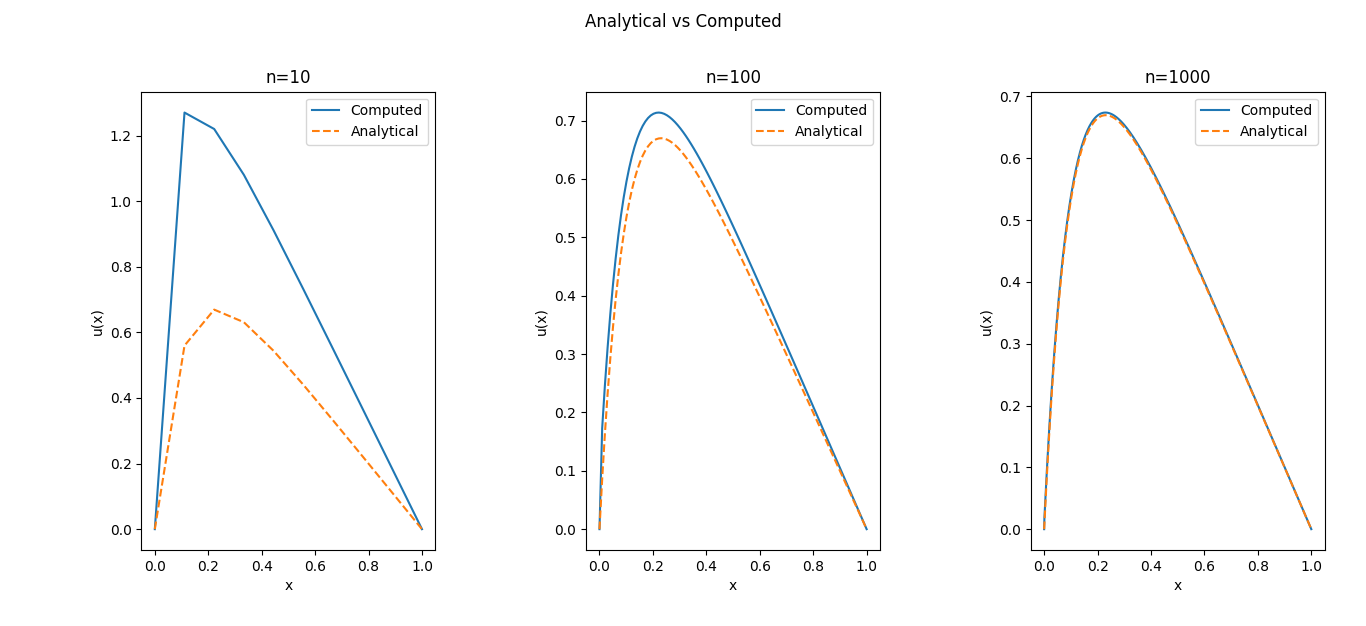
\includegraphics[width=\linewidth]{1b.png}
	\caption{Plot comparing analytical vs computed solutions of the differential equation. We can see that the computed solution approaches the analytical solution when the number of gridpoints increases.}
	\label{fig:1bplot}
\end{figure}
\subsection{Algorithm for specific tri-diagonal matrix}



 \subsection{Relative error}
 

  \subsection{LU decomposition}
 \begin{tabular}{ |p{4cm}||p{4cm}|p{4cm}|p{4cm}|  }
 \hline
 \multicolumn{4}{|c|}{Country List} \\
 \hline
Size & Generel algorithm& Special algorithm& LU decomposition \\ \\
 \hline
 n =10 & 0.00017 seconds & &0.585 seconds\\
n = 100 & 0.137 seconds   &  & 0.591 seconds\\
n = 1000 &0.146 seconds &  & 0.736 seconds\\
n = 10 000    &0.203 seconds&  &56.580 seconds\\
n = 100 000& 0.730 seconds & & ...\\
n = 1 000 000 & 6.177 secondss &    &...\\
 &  &  &\\
 \hline
\end{tabular}

  \section{Discussion}
    \subsection{LU decomposition}

 \begin{table}[h!]
\begin{center}
\caption{Relative error for specific tri-diagonal matrix algorithm.}
\begin{tabular}{ |c|c|c| } \hline
Steps (n)&Relative error ($\epsilon$) \\ \hline
$10$&$6.20*10^{-1}$ \\ \hline
$10^2$&$1.21*10^{-1}$ \\ \hline
$10^3$&$2.36*10^{-2}$ \\ \hline
$10^4$&$3.61*10^{-3}$ \\ \hline
$10^5$&$4.89*10^{-4}$ \\ \hline
$10^6$&$6.17*10^{-5}$ \\ \hline
$10^7$&$7.45*10^{-6}$ \\ \hline
\end{tabular}
\label{tab:e}
\end{center}
\end{table}
 
 \subsection{LU decomposition}



 \section{Discussion}
 
 We can see from table \ref{tab:e} that the relative error decreases as n increases. This is due to the fact that more grid points lead to better precision. However this is only true as long as we have enough memory to store our information. If we would increase the number of grid points further than $n=10^7$ our relative error could potentially increase dramatically. Since we are using python, more than $n=10^7$ grid points make the algorithm take too long to run. We could have used a larger n If we had used a faster programming language (like C++), making it possible to observe an increasing relative error at a larger n.\\
 \\
 \subsection{LU decomposition}
  If we compare our solution from the general algorithm and the CPU-time with the LU decomposition, we see that it takes a lot of more time to calculate the LU decomposition. This comes that it takes $n^3$ steps to find the LU decomposition, which is the same for gauss- elimination. But when we calculate LU decomposition, we calculate a set of two equation instead of one. This shows us that there are more steps for calculating just one vector. If we are going to calculate other vectors as well for the same matrix will show us that the LU decomposition will be much more effective. This comes from that we have already calculated the LU decomposition, which lead us to the calculation of the vector now is just $n^2$.    
\\
\\
The reason why we can’t use LU decomposition on a $10^5 \times 10^5$ matrix comes from the random accesses memory problem. The data that should be stored from the operation takes to much memory that the computer cant handle the operation we want to.  
\\

The number of floating point operations that the LU decomposition use to solve the set of linear equation equals $\frac{2}{3} n^3$. This means that the FLOPS depend on the size of the matrix. When the matrix becomes large, we can ignore the orders $n$ and $n^2$.     
  

The number of floating point operations that the LU decomposition use to solve the set of linear equation equals $\frac{2}{3} n^3$. This means that the FLOPS depend on the size of the matrix. When the matrix becomes large, we can ignore the orders $n$ and $n^2$.        

  
\section{Concluding remarks}




\bibliography{referanser}
\end{document}

